\documentclass[../Main.tex]{subfiles}
\setcounter{chapter}{15}

\begin{document}
\phantomsection
\chapter{L16: \texorpdfstring{$R$}{R}-module homomorphisms}
\begin{dfn}[title = {\texorpdfstring{$\Hom_R(M,N)$}{Hom}, Kernel, Image, Isomorphism}]
The \textbf{set of $R$-module homomorphisms from $M$ to $N$} is denoted $\Hom_R(M,N)$.\\
The \textbf{kernel} of an $R$-module homomorphism $f\in \Hom_R(M,N)$ is 
\[\Ker f \coloneqq \{m\in M \mid f(m)=0\}\]
The \textbf{image} of $f\in \Hom_R(M,N)$ is
\[\Img f \coloneqq \{n\in N\mid \exists m\in M, \, f(m)=n\}\]
If $f\in\Hom_R(M,N)$ is bijective then we say $f$ is an \textbf{isomorphism of $R$-modules}. We say $M,N$ are \textbf{isomorphic} if there is an isomorphism $f\colon M\to N$ and we write $M\cong N$.
\end{dfn}
\begin{example}
	$R=\Z,M=\Z$ is a $\Z$-module. \\
	\Note A subtle distinction between this and the ring of integers $\Z$ is that you don't have multiplication between the elements of the module but rather it has an action of the integers by multiplication.\\
	What do the $\Z$-module homomorphisms from $\Z$ to $\Z$ look like? Consider
	\begin{align*}
	f\colon \Z &\to \Z \\
	1&\mapsto a \\
	n&\mapsto \underbrace{a+a+a+\dots+a}_{n\text{-times}}
	\end{align*}
	Then we see that, in this case, $f$ is specified by where it sends one, i.e $f(1)=a$.
\end{example}
\Note There are functions $f$ which are $R$-module homomorphisms from $\Z $ to $\Z$ which are not ring homomorphisms from $\Z$ to $\Z$. Consider the doubling function
\begin{align*}
f_2\colon \Z&\to \Z \\
1&\mapsto 2
\end{align*}
is a $\Z$-module homomorphism as
\begin{align*}
f_2(m+n)&=2\rdot (m+n)=2\rdot m+2\rdot n = f_2(m)+f_2(n)\\
f_2(a\rdot m)&=2\rdot (a\rdot m) = a\rdot 2\rdot m = a\rdot f_2(m)
\end{align*}
However it is \textbf{not} a ring homomorphism as
\begin{align*}
f_2(2\rdot 3) = 2\rdot 2\rdot 3 =12 \ne 24 = 4\rdot 6 = (2\rdot 2) \rdot  (3\rdot 2) = f_2(2)\rdot f_2(3)
\end{align*}
\begin{prop}[title = Kernel and Image are submodules]
	Suppose $f\in \Hom_R(M,N)$. Then the kernel, $\Ker f \subset M$, and the image, $\Img f \subset N$,	 are $R$-submodules.
\end{prop}
\begin{proof}
	First we prove the claim for the kernel. If $a,b \in \Ker f$ and $r\in R$ then
	\begin{itemize}
	\item $f(0)=0\implies 0 \in \Ker f$
	\item $f(a+b) = f(a)+f(b) = 0 +0=0 \implies a+b \in \Ker f$
	\item$f(r\rdot a) = r\rdot f(a) = r\rdot 0=0 \implies r\rdot a \in \Ker f$
	\item$0=f(0)=f(a+(-a)) = f(a) + f(-a) = 0 +f(-a) = f(-a) \implies -a\in \Ker f$
	\end{itemize}
	hence, $\Ker f \subset M$ is a submodule.\\
	If $a,b\in \Img f, r\in R$ such that $a=f(a'), b=f(b')$ for $ a',b' \in M$, then
	\begin{itemize}
		\item $f(0)=0\implies 0\in \Img f$
		\item $a+b=f(a')+f(b')=f(a'+b')\implies a+b\in \Img f$
		\item $r\rdot a=r\rdot f(a')=f(r\rdot a') \implies r\rdot a \in \Img f$
		\item $-a=-f(a')=f(-a') \implies -a\in \Img f$
	\end{itemize}
	Hence, $\Img f$ is a submodule.
\end{proof}
\begin{dfn}[title = Coset]
	If $N\subset M$ is an $R$-submodule and $m\in M$, then the \textbf{$N$ coset} of $m$ is
	\[m+N \coloneqq \{m+n\mid n\in N\}\]
\end{dfn}
\Exr We can define an equivalence relation on $M$ by $m\sim m'$ if and only if $m+N = m'+N$ as sets.
\begin{center}
	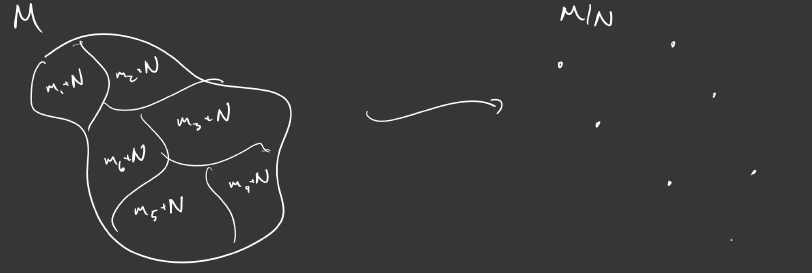
\includegraphics[width=0.8\textwidth]{coset}
\end{center}
\begin{dfn}[title = Quotient Module]
	The \textbf{quotient module} of $M$ by $N$ is
	\[M/N \coloneqq \{m+N \mid m\in M\}\]
\end{dfn}
\begin{prop}[title =Quotient Module is \texorpdfstring{$R$}{R}-module]
	Quotient modules are $R$-modules.
\end{prop}
\begin{proof}
	Define addition of cosets as 
	\[(m+N) + (m'+N) \coloneqq (m+m')+N\]
	Just as for rings, we will write $\obar{m}$ for $m\in M$ if $N$ is understood.\\
	It is simple enough to check that the addition is well defined:
	\begin{align*}
	m+N = m_1 + N \implies m-m_1=n \in N\\
	m'+N = m'_1 +N \implies m'-m'_1 = n' \in N
	\end{align*}
	Then by direct calculation
	\begin{align*}(m_1+N)+(m'_1+N) = (m+m'_1)+N =& (m+n+m'+n')+N\\ =& (m+m')+\underbrace{(n+n')}_{\in N} + N =(m+m')+N\end{align*}
	If $r\in R$ and $m+N \in M/N$. The $R$-action is then defined \[r\rdot (m+N) \coloneqq (r\rdot m)+N\] \Exr Check that the $R$-action is well defined.
\end{proof}
\begin{prop}[title = Canonical quotient map is surjective]
	The natural quotient map
	\begin{align*}
	p\colon M \to& M/N \\
	m\mapsto& M+N
	\end{align*}
	is a surjective $R$-module homomorphism such that $\Ker p= N$.
\end{prop}
\begin{proof}
	Properties of an $R$-module homomorphism:
	\begin{align*}
	&p(a+b)=(a+b)+N=(a+N)+(b+N)=p(a)+p(b)\\
	&p(r\rdot a)=(r\rdot a)+N = r\rdot (a+N) = r\rdot p(a)
	\end{align*}
	Surjectivity is clear as before (think of the representative of the coset).\\
	Suppose $a\in \Ker p$, then $f(a) = a+N = 0+N$ i.e. there exists $n\in N$ such that $a-0=n\in N$ and hence $a=n\in N$ so that $a\in N$. Hence, $\Ker p \subset N$.
	Suppose $n\in N$. Then
	\[f(n)=n+N \implies n-0\in N \implies n+N = 0+N \implies f(n) = 0+N \implies n\in \Ker p\]
	and therefore $N \subset \Ker p$. 
\end{proof}

\begin{thm}[title = The First Isomorphism Theorem]
	Let $M,N$ be $R$-modules and $f\in \Hom_R(M,N)$. Then $\Ker f \subset M$ is a submodule and
	\[M/\Ker f \cong \Img f\]
\end{thm}
\begin{thm}[title = The Second Isomorphism Theorem]
	Let $A,B\subset M$ be submodules, then
	\[(A+B)/B \cong A/A\cap B\]
\end{thm}
\begin{thm}[title = The Third Isomorphism Theorem]
Let $A\subset B\subset M$ be submodules, then
\[(M/A)/(B/A) \cong M/B\]
\end{thm}
\begin{thm}[title = The Fourth Isomorphism Theorem]
	There is a bijection of sets
	\[\{ \text{submodules of } M \text{ containing } N \} \longleftrightarrow \{ \text{submodules of } M/N \}\]
	\center
	\begin{tikzcd}[column sep=0em,row sep=1em]
		&M\arrow[dl,dash]\arrow[dr,dash] &&&&& M/N\arrow[dl,dash]\arrow[dr,dash]\\
		A\arrow[dr,dash] && B\arrow[dl,dash] \arrow[rrr, leftrightarrow] % This is the new bit
		&\phantom{X}\arrow[r,dash]&\phantom{Y}& A/N\arrow[dr,dash] && B/N\arrow[dl,dash]\\
		&C\arrow[d,dash] &&&&& C/N\arrow[d,dash]\\
		&N &&&&& 0
	\end{tikzcd} 
\end{thm}
\begin{prop}[title = \texorpdfstring{$\Hom_R(M,N)$}{Hom} is an \texorpdfstring{$R$}{R}-module]
	Suppose $M,N$ are $R$-modules, then $\Hom_R(M,N)$ is itself an $R$-module
\end{prop}
\begin{proof}
	Define addition for $f,g\in \Hom_R(M,N)$ as
	\[(f+g)(m)\coloneqq f(m)+g(m)\]
	\Exr Check that
	\begin{align*}
	0\colon M&\to N\\
	m&\mapsto 0
	\end{align*}
	is the additive identity and
	\begin{align*}
	-f\colon M&\to N\\
	m&\mapsto -f(m)
	\end{align*}
	is the additive inverse. Thus it is shown that $\Hom_R(M,N)$ is an abelian group with the binary operation $+$.\\
	Then the $R$-action for $r\in R$ and $f\in \Hom_R(M,N)$ is
	\begin{align*}
	(r\rdot f)\colon M &\to N\\
	m&\mapsto r\rdot f(m)
	\end{align*}
	\Exr Check that $\Hom_R(M,N)$ satisfies all the $R$-module action properties.
\end{proof}
\newpage
\Note These operations are the same operations one learns for functions in middle school (even linear transformations in Linear Algebra):
\[f\colon \R^n \to \R^m\]
This can be seen by the following
\begin{align*}
&\begin{pmatrix}
a&b\\
c&d
\end{pmatrix} + \begin{pmatrix}
e&f\\
g&h
\end{pmatrix} = \begin{pmatrix}
a+e&b+f\\
c+g&d+h
\end{pmatrix}\\
&\alpha \begin{pmatrix}
a&b\\
c&d
\end{pmatrix} = \begin{pmatrix}
\alpha a&\alpha b\\
\alpha c&\alpha d
\end{pmatrix}
\end{align*}
But there is one additional operation that you can preform with homomorphisms which can not be performed by elements of the module, and that is function composition.
\begin{prop}
	If $f\in \Hom_R(M,N), g \in \Hom_R(N,L)$ then $g\circ f \colon M\to L$ and $g\circ f \in \Hom_R(M,L)$
\end{prop}
\begin{proof}
	Shown by direct check of homomorphism properties
	\begin{align*}
	&g\circ f(x+y) = g(f(x+y)) = g(f(x)+f(y)) = g(f(x)) +g(f(y)) =g\circ f(x) + g\circ f(y)\\
	&g\circ f(a\rdot x) = g(f(a\rdot x)) = g(a\rdot f(x)) = a\rdot g(f(x))=a\rdot g\circ f(x) \qedhere
	\end{align*}
\end{proof}
In particular, if $M=N=L$, then $f,g \in \Hom_R(M,M)$ and $g\circ f \in \Hom_R(M,M)$, i.e. you stay in the same set by composition if the domain and range are the same set. This leads naturally to the following observation
\begin{crl}[title=\texorpdfstring{$\Hom_R(M,M)$}{Hom} is a ring]
	$\Hom_R(M,M)$ is a ring with $1$. In this ring, addition are $f+g$ and multiplication as composition $f\circ g$.
\end{crl}
\begin{proof}
	We know $(\Hom_R(M,M),+)$ is an abelian group.\\
	It remains to check that composition is/has \\
	(\textbf{Associativity})
		\[[(f\circ g) \circ h](x) = (f\circ g)[h(x)] = f[g(h(x))] = f[(g\circ h)(x)] = [f\circ (g\circ h)](x)\]
	(\textbf{Distributivity over $+$})
		\[[f\circ (g+h)](x) = f[(g+h)(x)] = f[g(x)+h(x)] = f(g(x)) +f(h(x)) = (f\circ g)(x) + (f\circ h)(x)\]
	(\textbf{Identity})
		The identity map is simply given by
		\begin{align*}
		\Id \colon M&\to M \\
		m&\mapsto m
		\end{align*}
		\Exr Check that this is truly the identity for composition.
\end{proof}
\begin{dfn}[title = Endomorphisms and Endomorphism Ring]
	The ring $\Hom_R(M,M)$ is called the \textbf{endomorphism ring} of $M$. We sometimes denote it by $\End_R(M)$.\\
	The elements of $\End_R(M)$ are \textbf{endomorphisms}.
\end{dfn}
\begin{example}
	If $M$ is any $R$-module and $a\in R$ where $R$ is commutative, then we can define
	\begin{align*}
	a\rdot \Id \colon M &\to M \\
	m&\mapsto a\rdot m
	\end{align*}
	is an endomorphism.
	\begin{proof}
		Simply check homomorphism properties
	\begin{align*}
	&(a\rdot \Id)(m+n)\coloneqq a\rdot (m+n) = a\rdot m + a\rdot n = (a\rdot \Id)(m) + (a\rdot \Id)(n)\\
	&(a\rdot \Id)(r\rdot m) \coloneqq a\rdot (r\rdot m) = (ar )\rdot m = (r a)\rdot m = r\rdot (a\rdot m) = r\rdot (a\rdot \Id)(m) \qedhere
	\end{align*}
	\end{proof}
\end{example}
This leads naturally the the following map from the ring $R$ to the endomorphisms:
\begin{align*}
f\colon R&\to \End_R(M)\\
r&\mapsto r\rdot \Id
\end{align*}
\begin{claim}
	This map is a ring homomorphism.
\end{claim}
\begin{proof}
	We check ring homomorphism properties for $r,s\in R$
	\begin{align*}
	&f(r+s)\coloneqq (r+s)\rdot \Id = r\rdot \Id + s\rdot \Id = f(r)+f(s)\\
	&f(r s) = {\color{blue}{(r s)\rdot \Id = (r\rdot \Id) \circ (s\rdot \Id)}} = f(r)\rdot f(s)\qedhere
	\end{align*}
	The equality in blue can be seen by evaluating at $m\in M$,
	\[[(r s)\rdot \Id](m)=(r s)\rdot m = r\rdot (s\rdot m)= r\rdot (s\rdot \Id)(m) = (r\rdot \Id)\circ (s\rdot \Id)(m) \qedhere \]
\end{proof}
\textbf{\textcolor{BrickRed}{\underline{Warning}}}: This map is not always injective as seen by the following example:
\begin{example}
	$\modZ{4}$ is a $\Z$-module and so consider the map
	\begin{align*}
	f\colon \Z&\to \End(\modZ{4}) \\
	4&\mapsto 4\rdot \Id
	\end{align*}
	However we can see that $\Ker f$ does not contain only $0$,
	\[4\rdot \Id(\obar{a}) = 4\rdot \obar{a} = \obar{4a} = \obar{0} \implies 4 \in \Ker f\]
	Hence, $f$ is not injective.
\end{example}
\end{document}